\documentclass[]{book}
\usepackage{lmodern}
\usepackage{amssymb,amsmath}
\usepackage{ifxetex,ifluatex}
\usepackage{fixltx2e} % provides \textsubscript
\ifnum 0\ifxetex 1\fi\ifluatex 1\fi=0 % if pdftex
  \usepackage[T1]{fontenc}
  \usepackage[utf8]{inputenc}
\else % if luatex or xelatex
  \ifxetex
    \usepackage{mathspec}
  \else
    \usepackage{fontspec}
  \fi
  \defaultfontfeatures{Ligatures=TeX,Scale=MatchLowercase}
\fi
% use upquote if available, for straight quotes in verbatim environments
\IfFileExists{upquote.sty}{\usepackage{upquote}}{}
% use microtype if available
\IfFileExists{microtype.sty}{%
\usepackage{microtype}
\UseMicrotypeSet[protrusion]{basicmath} % disable protrusion for tt fonts
}{}
\usepackage[margin=1in]{geometry}
\usepackage{hyperref}
\hypersetup{unicode=true,
            pdftitle={A Minimal Book Example},
            pdfauthor={Yihui Xie},
            pdfborder={0 0 0},
            breaklinks=true}
\urlstyle{same}  % don't use monospace font for urls
\usepackage{natbib}
\bibliographystyle{apalike}
\usepackage{longtable,booktabs}
\usepackage{graphicx,grffile}
\makeatletter
\def\maxwidth{\ifdim\Gin@nat@width>\linewidth\linewidth\else\Gin@nat@width\fi}
\def\maxheight{\ifdim\Gin@nat@height>\textheight\textheight\else\Gin@nat@height\fi}
\makeatother
% Scale images if necessary, so that they will not overflow the page
% margins by default, and it is still possible to overwrite the defaults
% using explicit options in \includegraphics[width, height, ...]{}
\setkeys{Gin}{width=\maxwidth,height=\maxheight,keepaspectratio}
\IfFileExists{parskip.sty}{%
\usepackage{parskip}
}{% else
\setlength{\parindent}{0pt}
\setlength{\parskip}{6pt plus 2pt minus 1pt}
}
\setlength{\emergencystretch}{3em}  % prevent overfull lines
\providecommand{\tightlist}{%
  \setlength{\itemsep}{0pt}\setlength{\parskip}{0pt}}
\setcounter{secnumdepth}{5}
% Redefines (sub)paragraphs to behave more like sections
\ifx\paragraph\undefined\else
\let\oldparagraph\paragraph
\renewcommand{\paragraph}[1]{\oldparagraph{#1}\mbox{}}
\fi
\ifx\subparagraph\undefined\else
\let\oldsubparagraph\subparagraph
\renewcommand{\subparagraph}[1]{\oldsubparagraph{#1}\mbox{}}
\fi

%%% Use protect on footnotes to avoid problems with footnotes in titles
\let\rmarkdownfootnote\footnote%
\def\footnote{\protect\rmarkdownfootnote}

%%% Change title format to be more compact
\usepackage{titling}

% Create subtitle command for use in maketitle
\newcommand{\subtitle}[1]{
  \posttitle{
    \begin{center}\large#1\end{center}
    }
}

\setlength{\droptitle}{-2em}
  \title{A Minimal Book Example}
  \pretitle{\vspace{\droptitle}\centering\huge}
  \posttitle{\par}
  \author{Yihui Xie}
  \preauthor{\centering\large\emph}
  \postauthor{\par}
  \predate{\centering\large\emph}
  \postdate{\par}
  \date{2017-12-05}


\begin{document}
\maketitle

{
\setcounter{tocdepth}{1}
\tableofcontents
}
\clearpage

\chapter{Introduction}\label{introduction}

Edwin Herbert Hall discovered the ``Hall effect'' in 1879 while working
on his doctoral thesis in Physics investigating the influence of magnets
on the resistance of a coil excited by a current. Hall discovered that a
magnetic field would skew equipotential lines in a current-carrying
conductor. This effect is observed as a voltage (Hall voltage)
perpendicular to the direction of the current in the conductor.

The magnitude of this discovery is even more impressive considering how
little was known about electricity in his time. The electron, for
instance, was not identified until more than 10 years later.

The ``Hall effect'' remained a laboratory curiosity until the latter
half of the XX century because the materials available, such as metals,
would only produce small Hall voltages. With the advent of semiconductor
technology and the development of various III-V compounds, it became
possible to produce Hall voltages many orders of magnitude greater,
allowing the production of Hall sensors, mostly made of indium
antimonide (\(\mathrm{InSb}\)), indium arsenide (\(\mathrm{InAs}\)) and
gallium arsenide (\(\mathrm{GaAs}\)).

\chapter{A macroscopic approach to Ohm's
laws}\label{a-macroscopic-approach-to-ohms-laws}

The usual \emph{macroscopic} approach to electrical conduction is based
on the following experimental observations on metallic conductors:

\begin{enumerate}
\def\labelenumi{\arabic{enumi})}
\item
  The application of a steady voltage difference \(V\) to a metallic
  wire produces a steady electric current \(I\) proportional to \(V\).
  This holds true at least for small values of \(I\) when the
  temperature of the wire does not increase appreciably.

  This allows the definition of the \emph{electric resistance} as
  follows, according to the first Ohm's law:

  \begin{equation}
   R=\frac{ V }{ I }
   \label{eq:ohmLaw1}
   \end{equation}
\item
  For high currents the wire temperature increases and the power
  \(W=VI\) supplied by the generator to the moving charges, instead of
  accelerating more and more the circulating charge, is converted into
  heat (Joule effect).

  It could appear that the moving charges are subjected to some kind of
  force, like a body falling in a viscous medium, so that they reach a
  steady motion and give up part of their kinetic energy to the ``body''
  of the wire (i.e.~to the crystal lattice).
\item
  The resistance \(R\) increases with increasing temperature.
\item
  Using wires of different length \(l\) and sections \(S\) the second
  Ohm's law determines the resistance:
\end{enumerate}

\begin{equation}
R= \frac{ \rho l}{S} 
\label{eq:ohmLaw2}
\end{equation}

where the constant \(\rho\) (the \emph{electrical resistivity}) has a
characteristic value for any material and increases with temperature.

The inverse quantity, the \emph{electrical conductivity} \(\sigma\), can
be expressed using the two Ohm's laws as:

\begin{equation}
\sigma = \frac{1}{ \rho }=\frac{J}{E}
\label{eq:conductivity}
\end{equation}

where \(J\) is the current density and \(E\) the electric field
intensity. This is the starting relation needed to pass to a
\emph{microscopic} picture, that will allow a better understanding of
the phenomena.

\chapter{A semiclassical microscopic
model}\label{a-semiclassical-microscopic-model}

The simplest microscopic model one can use is the ``free electron gas''
model of metals, in which the valence electrons are supposed to be
practically free from their original atoms, and thus to move in the
crystal lattice formed by the metal ions. In the absence of an applied
electric field, the electron velocities are randomly distributed, with
zero mean value and a \emph{root mean square} value \(v_{m}\) that may
be evaluated from the equation:

\begin{equation}
\frac{1}{2}mv_{m}^2=\frac{3}{2}kT
\label{eq:electronVrms}
\end{equation}

where \(k\) is the Boltzmann constant, \(m\) the electron mass and \(T\)
the absolute temperature: at room temperature \(v_{m}\) turns out to be
of the order of \(10^5 m/s\).

Only when an electric field is externally applied the electron motion
acquires an ordered component with a \emph{mean value} \(v_d\) (the
\emph{drift velocity}) which turns out to be very small with respect to
\(v_{m}\) as we will show later.

The drift velocity, i.e.~this ordered component of the motion due to the
electric field and to the the scattering of the electrons with the
lattice, is simply proportional to the electric field intensity. The
constant ratio between \(v_d\) and \(E\) (both in modulus) is called the
\emph{drift mobility} \(\mu\).

During a time \(t\) of free motion between two collisions,the electrons
subject to the force \emph{qE} (\emph{q} is the electron charge)
increase their speed of the quantity:

\begin{equation}
a t = \frac{qE}{m}t
\label{eq:electronsDelta}
\end{equation}

The kinetic energy of the electrons also increases, but it can be
assumed that with each collision they lose additional energy. The
transfer of such energy to the lattice ions explains the Joule effect.

It can be noticed\footnote{See for instance \emph{The Feynman lectures
  on Physics} vol.I 43-1,3 Addison-Wesley 1963.} that, after the
application of the electric field, the average speed of the electrons is
not zero but instead:

\begin{equation}
v_d=a\tau=q\tau\frac{E}{m}
\label{eq:electronsAvgSpd}
\end{equation}

obtained from \eqref{eq:electronsDelta} where \(\tau\) is the mean free
time between collisions \footnote{This time \(\tau\) does not depend on
  the electric field because the average speed increment due to the
  applied electric field \(V_d\) is very small with respect to the
  r.m.s. speed \(V_m\) due to thermal motion .}, so that the drift
mobility \(\mu\) has the microscopic expression :

\begin{equation}
\mu = \frac{v_d}{E} = \frac{q\tau}{m}
\label{eq:driftmobility}
\end{equation}

Using these concepts of drift speed and mobility the current density
\(J\) can be written as:

\begin{equation}
J = qn v_d
\label{eq:currentDensity}
\end{equation}

where \(n\) is the free electron concentration and relation
\eqref{eq:conductivity} and \eqref{eq:driftmobility} allow us to give a
\emph{microscopic definition} of the electrical conductivity:

\begin{equation}
 \sigma = q n \mu 
\label{eq:electricalConductivity}
\end{equation}

Relation \eqref{eq:electricalConductivity} tells us that all the physics
of electrical conduction is described by the two parameters \(n\) and
\(\mu\).

In the electron gas model \(n\) should be, for a monovalent metal:

\begin{equation}
n=\frac{N_Am}{\delta}
\label{eq:nmonovalentmetal}
\end{equation}

where \(N_A\) is Avogadro's number, \(m\) is the atomic mass and
\(\delta\) the density. As an example \(n=8.5 \cdot 10^{28}m^{-3}\) for
copper. Of course here \(n\) does not depend on the temperature, while
drift mobility decreases with increasing temperature\footnote{Drift
  mobility in semiconductors decreases with the absolute temperature
  \(T\) as \(T^{-\alpha }\), where \(1.5<a<3.0\) depending on the
  prevailing type of interactions of the free carriers (with phonons,
  lattice defects, or impurities).} because of the increased thermal
vibrations of the lattice ions.

A rough order of magnitude for the electron mobility may be derived
using \eqref{eq:driftmobility}. A reasonable value for \(\tau\) is:
\(\tau\approx\lambda/v_{m}\), where \(\lambda\) is the electron mean
free path, of the order of the interatomic distance in the metal (i.e.~a
few \(\mathring{A}\)) so that, at room temperature, \(\tau\) is of the
order of \(10^{-15}s\).

Using the values of the elementary charge \(e = 1.6 \cdot 10^{-19 }C\)
and of the electron mass \(9 \cdot 10^{-28} g\), the electron mobility
\(\mu=\frac{e\tau}{m}\) should be of the order of some
\(\frac{cm^2}{Vs}\).

Even for very large electric fields (up to \(10^2 \frac{V}{cm}\)) the
drift velocity \(v_d=\mu E\) is thus much smaller than \(v_{m}\).

In order to check experimentally the microscopic model we must measure
not only the electrical resistance (which gives the product of \(n\) and
\(\mu\)) but also the free charge density \(n\): this can be obtained by
performing a measurement of the Hall effect.

\chapter{The Hall effect}\label{the-hall-effect}

The Hall effect is essentially due to the Lorentz force \(\vec { F }\)
acting on each electric charge \(q\) moving with velocity \(v\) in a
magnetic field \(B\).

\begin{equation}
\vec { F } =q\vec { V } \wedge \vec { B }
\label{eq:lorentzForce}
\end{equation}

Let us consider a conducting bar (Fig. \ref{fig:hall-effect-geometry})
immersed into a uniform magnetic field \(B\) directed along the \(z\)
axis, with an electric current \(I_x\) flowing along the \(x\) axis. The
Lorentz force \(F_L\) on moving charges, both positive and negative,
acts in the direction shown by the arrow (Fig.
\ref{fig:hall-effect-geometry}) (independently from the charge sign).

\begin{figure}

{\centering 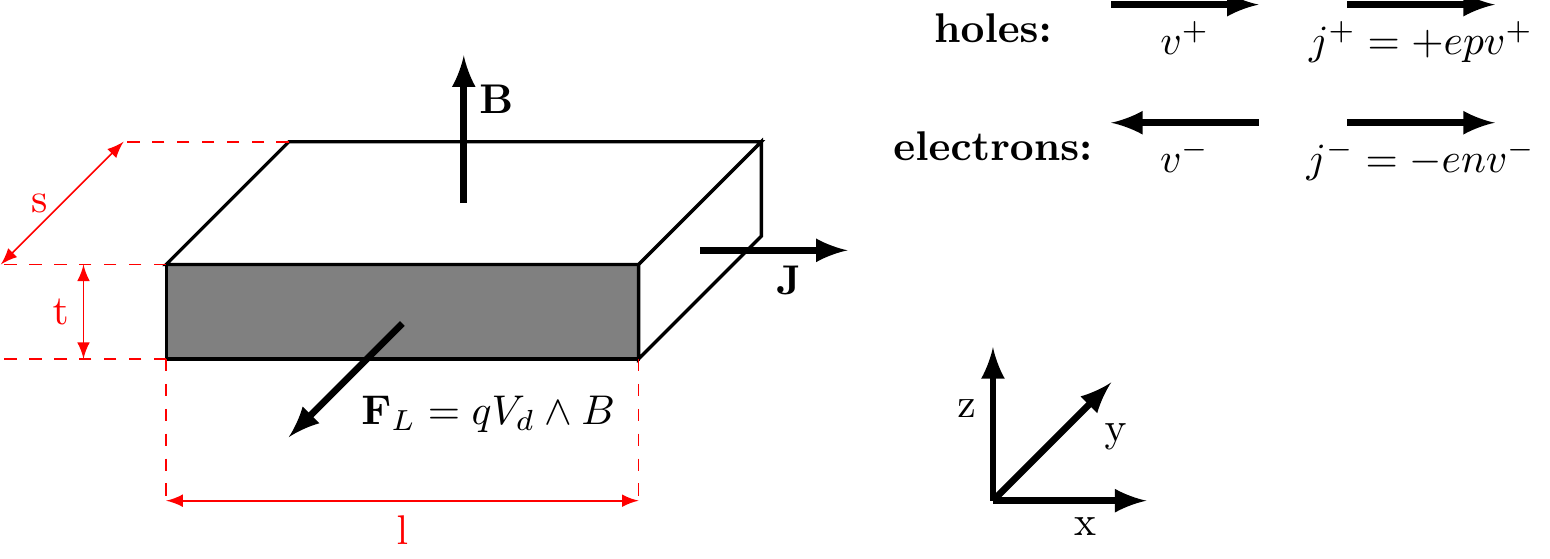
\includegraphics[width=0.65\linewidth]{Assets/Figures/hall-effect-geometry} 

}

\caption{Hall effect geometry}\label{fig:hall-effect-geometry}
\end{figure}

In metals the electric current is only due to electrons. In
semiconductors the charge carriers may be either electrons or holes.

In a pure semiconductor the electron density \(n\) and the hole density
\(p\) is identical, in doped semiconductor we have \(n\gg p\) (in
N-doped material) or \(p\gg n\) (in P-doped material). In doped
semiconductors only one type of charge carriers is therefore important.

Let us consider first a metal or a N-doped semiconductor sample, where
the relevant charge carriers are electrons.

In the electric field \(E_x\) the electrons gain a drift velocity
\(v_d=–\mu E_x\) and they are subject to the Lorentz force
\(F_L=qv_dB\), pointing towards the negative \(y\). While drifting in
the \(x\) direction they tend to crowd at the sample surface orthogonal
to the \(y\) axis and placed towards the reader in Fig.
\ref{fig:hall-effect-geometry}.

This charge density increase at the sample lateral surface produces a
difference of potential along the \(y\) axis and therefore an electric
field \(E_H\). The value of the \emph{Hall field} \(E_H\) at equilibrium
will correspond to an electric force \(qE_H\) equal and opposite to the
Lorentz force, i.e. \(E_H=v_d B\). This relation tells us that the Hall
field is proportional both to the current density (through \(v_d\)) and
to the magnetic field. It is therefore convenient to define the Hall
coefficient as:

\begin{equation}
R_H=\frac{E_H}{J_x B_z}
\label{eq:hallCoefficient}
\end{equation}

Recalling the relations \(J_x=-env_d\) (or \(J_x=+epv_d\)) we get :

\begin{equation}
R_{ H }=V_{ d }\frac { B }{ J_{ x }B } =\frac { -1 }{ en } 
\label{eq:RHmn}
\end{equation}

or otherwise, for P-doped conductors:

\begin{equation}
 R_{ H }=\frac { +1 }{ ep }
\label{eq:RHp}
\end{equation}

Depending on the type of conductor, either metal
\eqref{eq:hallCoefficient} , N-doped \eqref{eq:RHmn} or P-doped
\eqref{eq:RHp}.

Measuring \(R_H\) we can determine the concentration \(n\) of majority
carriers and their sign (if we know the direction of the vectors
\(\vec { B } ,\vec { J } ,\vec { E_{ h } }\) ).

We can obtain relation \eqref{eq:RHmn} by assuming identical drift
velocity for all charge carriers. This is an approximate relation, found
in the literature:

\begin{equation}
 R_H = \frac{r}{nq}
\label{eq:foundInLiterature}
\end{equation}

where \(r\) is a parameter that accounts for the statistical velocity
distribution of the charge carriers, as well as the different scattering
mechanisms: \(r\approx 1.2\) for mainly phonon scattering (lattice
vibrations) and \(r\approx 1.9\) for mainly impurity scattering.

The Hall coefficient in semiconductors is many order of magnitude larger
than the one in metals, due to the smaller charge density. This makes
easier to measure Hall voltages in semiconductors, where a bias current
\(I_x\) of a few \(mA\) may conveniently generate a Hall voltage \(V_H\)
of in the order of a few \(mV\).

To measure \(R_H\) we must know \(V_H\), \(I_x\), \(B\) and the sample
thickness \(t\):

\begin{equation}
 R_{ H }=\frac { E_{ h } }{ B{ J }_{ x } } =\frac { V_{ H } }{ s } =\frac { B{ I }_{ x } }{ ts } =\frac { V_{ h }t }{ B{ I }_{ x } } 
\label{eq:Rh}
\end{equation}

It is worth noting that the the Lorentz force direction does not depend
on the charge sign.

The general expression for \(R_H\), valid (see Appendix 1) when
\emph{both electrons and holes} are present with densities \(n\) and
\(p\) and mobility \(\mu_e\) and \(\mu_h\) is:

\begin{equation}
 R_{ H }=r\frac { p\mu ^{ 2 }_{ h }-n\mu ^{ 2 }_{ e } }{ e(p\mu _{ h }-n\mu _{ e })^{ 2 } } 
\label{eq:RhGeneralExpression}
\end{equation}

Which corresponds to the relations and \eqref{eq:RHmn} and \eqref{eq:RHp}
for \(p\gg n\) or \(n\gg p\)

When two types of charge carriers are present the electrical
conductivity becomes:

\begin{equation}
\sigma =e(p \mu_h + n \mu_e)
\label{eq:electricalConductivity2Carriers}
\end{equation}

The product \(R_H \sigma\), is named Hall mobility \(\mu_H\) (note the
capital index ``\(H\)'' that distinguish it from hole mobility
\(\mu_h\)).

For a doped semiconductor the Hall mobility \(\mu_H\) approximates the
\emph{majority carriers} drift mobility \(\mu_{h,e}\):

\begin{equation}
\mu _{ H }=R_{ H }\sigma =r\frac { p \mu^2_h - n \mu^2_e }{p \mu_h + n \mu_e} \approx r \mu_{h,e} 
\label{eq:muApproximateDriftMobility}
\end{equation}

From relation \eqref{eq:RhGeneralExpression} we see that by increasing the
temperature in a \emph{P-doped sample}, generating many
intrinsic\footnote{\emph{Intrinsic} term labels properties related to
  pure semiconductors or to doped semiconductors at hight temperature,
  where the thermally generated carriers density is much larger than the
  (\emph{extrinsic}) carrier density due to the dopant.} carriers
(i.e.~electron-hole pairs), the Hall coefficient \(R_H\) (which is
positive at room temperature in the extrinsic region) tends to decrease,
and it may even change sign. This is explained by the mobility ratio
\(b=\mu_e/\mu_h>1\). \emph{Note that this does not happen with a}
N\emph{-doped sample}.

From relation \eqref{eq:RhGeneralExpression} at the temperature where
\(R_H=0\) (``\emph{inversion point}'') we get \(nb^2=p\), with
\(p=N_a+N\) and \(n=N\) (where \(N_a\) is the dopant density and \(N\)
is the thermally-generated charge density in the intrinsic zone).
Therefore \(Nb^2= N_a+N\), or \(N_a/N=b^2-1\).

The intrinsic conductivity \emph{measured} at the inversion point is:

\begin{equation}
\sigma_{oi} = e(n \mu_e + p \mu_h ) = e[N( \mu_e + \mu_h)+ N_a \mu_h ] = e \mu_h [N(b+1)+N_a]
\label{eq:intrinsicConductivityInvPoint}
\end{equation}

In the extrinsic region of a P-doped sample, where the charge carrier
density is constant \(n=N_a\), the conductivity is proportional to the
carrier mobility \(\mu_h\): i.e. \(\sigma_e(T) = eN_a \mu_h(T)\)

The experimentally measured temperature dependence of the mobility is a
power-law \(\mu(T)=const( T^\alpha)\), where the exponent \(\alpha\) (in
the range \(1.5<\alpha<3.0\)) depends on the type of prevailing
interaction of the charge carriers with phonons, lattice defects or
impurities).

Therefore we may \emph{extrapolate the extrinsic conductivity at the
inversion point} \(\sigma_{ei}\), and from the ratio
\({\sigma_{oi}}/{\sigma_{ei}}\) we get the \(b\) value:

\begin{equation}
\frac{\sigma_{oi}}{\sigma_{ei}} =e\mu_h \frac{N(b+1) + N_a}{e N_a \mu_h}= \frac{b}{b-1}
\label{eq:extrinsicConductivityInvPoint}
\end{equation}

which can as well be written as:

\begin{equation}
b=\frac{R_e}{R_e-R_o}
\label{eq:extrinsicConductivityInvPoint2}
\end{equation}

where \(R_o\) is the measured sample resistance at the inversion point
and \(R_e\) is the resistance extrapolated from the extrinsic region
(low temperature) to the value it would have at the inversion
temperature.

The dopant concentration is related to the value of the \emph{Hall
constant at the inversion point} \(R_{Ho}\) (in the extrinsic region
only the hole concentration is significant) by the equations
\eqref{eq:RHmn} and \eqref{eq:RHp}, i.e. :

\begin{equation}
N_a \approx p \approx \frac{1}{e R_{Ho}}
\label{eq:HallConstantInvPointRelation}
\end{equation}

\chapter{Experiment Procedure}\label{experiment-procedure}

\section{The experimental setup}\label{the-experimental-setup}

The apparatus uses a Ge sample, cut from a standard P-doped wafer,
placed inside a isothermal aluminum case. It is placed in the gap
between two poles of a permanent magnet, realized from two Nd-Fe-B
magnets and a U shaped soft-steel core, acting like a torus.

The sample has 7 wires tin soldered in the positions shown in Fig.
\ref{fig:sample-circuitry} and Fig. \ref{fig:sample-pcb} as follows:

\begin{figure}

{\centering 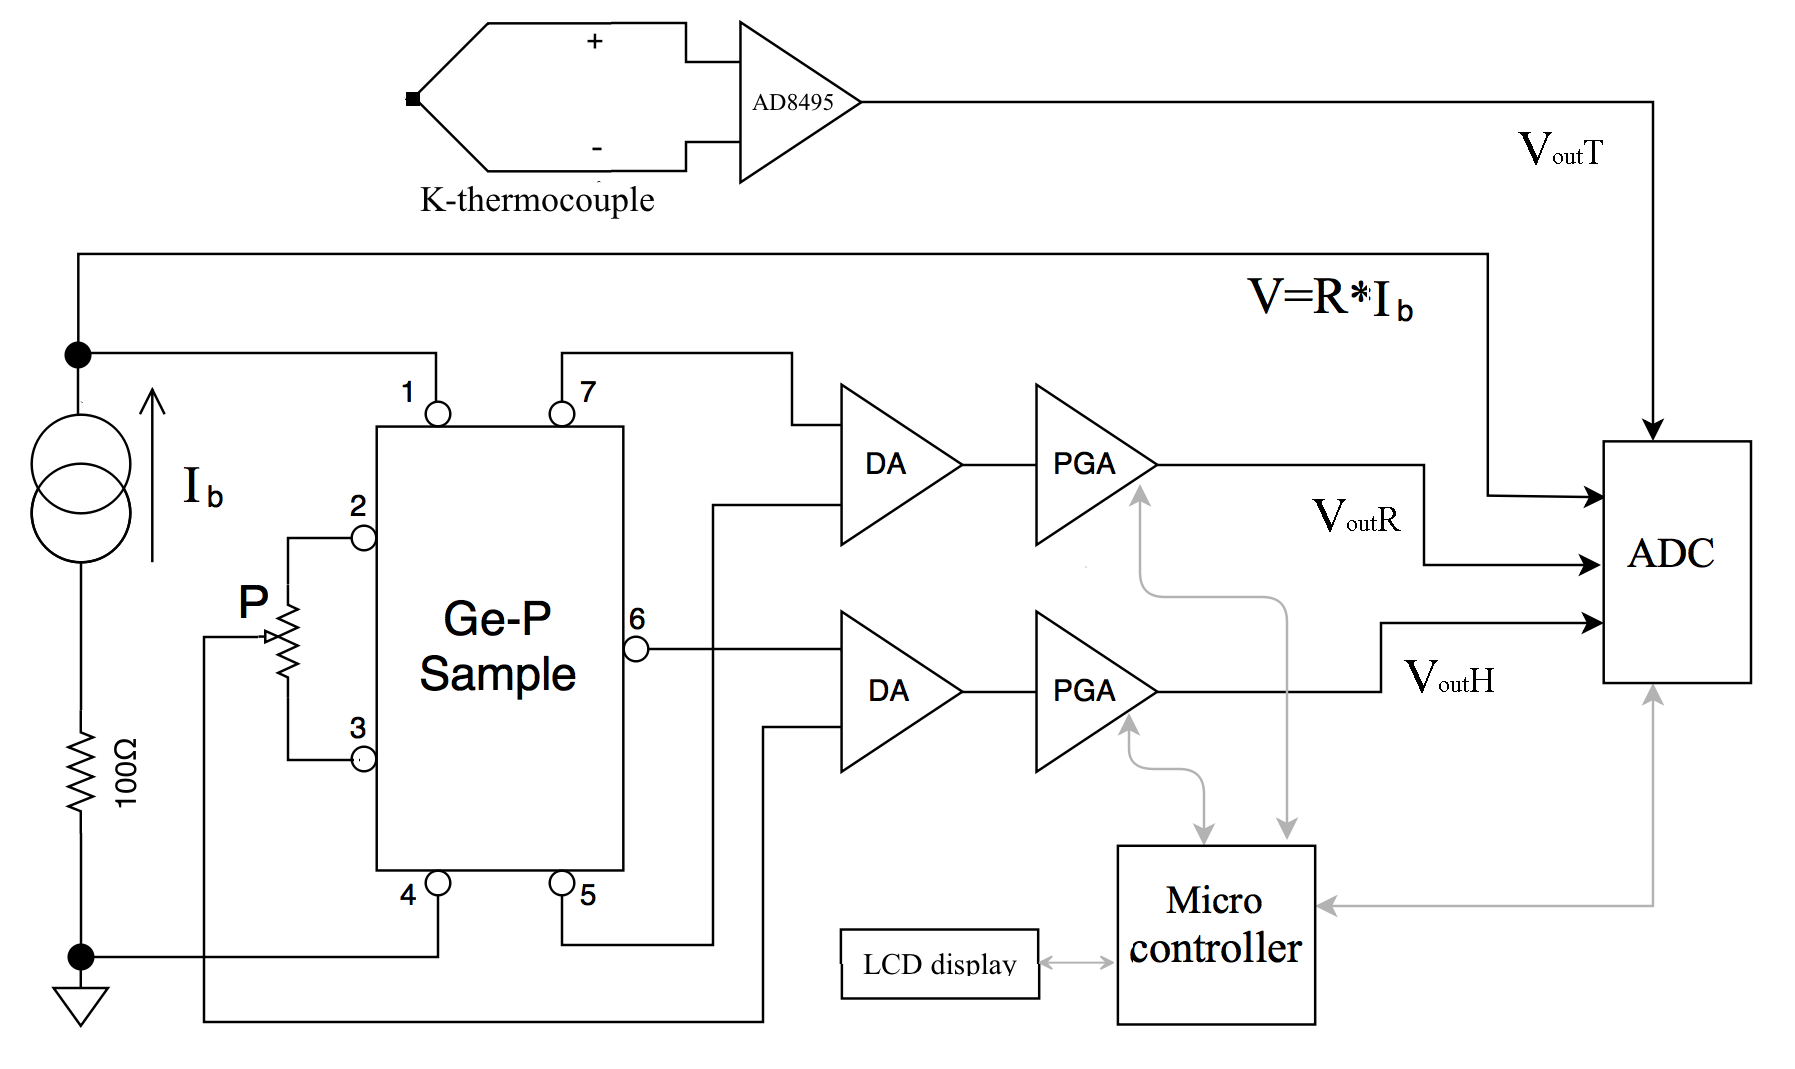
\includegraphics[width=0.65\linewidth]{Assets/Figures/sample_circuitry} 

}

\caption{Simplified schematic of the sample circuitry}\label{fig:sample-circuitry}
\end{figure}

\begin{itemize}
\item
  Contacts 1 and 4 are used to feed the bias current Ib produced by a
  constant current generator (Fig. \ref{fig:sample-circuitry}).
\item
  Contacts 7 and 5 are used to measure (through a differential
  amplifier, DA for short) the voltage across the sample, in a 4-wire
  resistance measurement.
\item
  Contacts 2-3 and 6 are the output of the Hall voltage and fed to the a
  second DA.

  Contact 6 is the reference point for the Hall voltage and contacts 2
  and 3 are used to set the balancing potentiometer P after having
  removed the sample from the magnetic field (the Hall voltage should be
  zero in absence of applied magnetic field). \emph{Three contacts} are
  needed for the Hall voltage because \emph{two contacts} cannot be
  precisely aligned.
\end{itemize}

\begin{figure}

{\centering 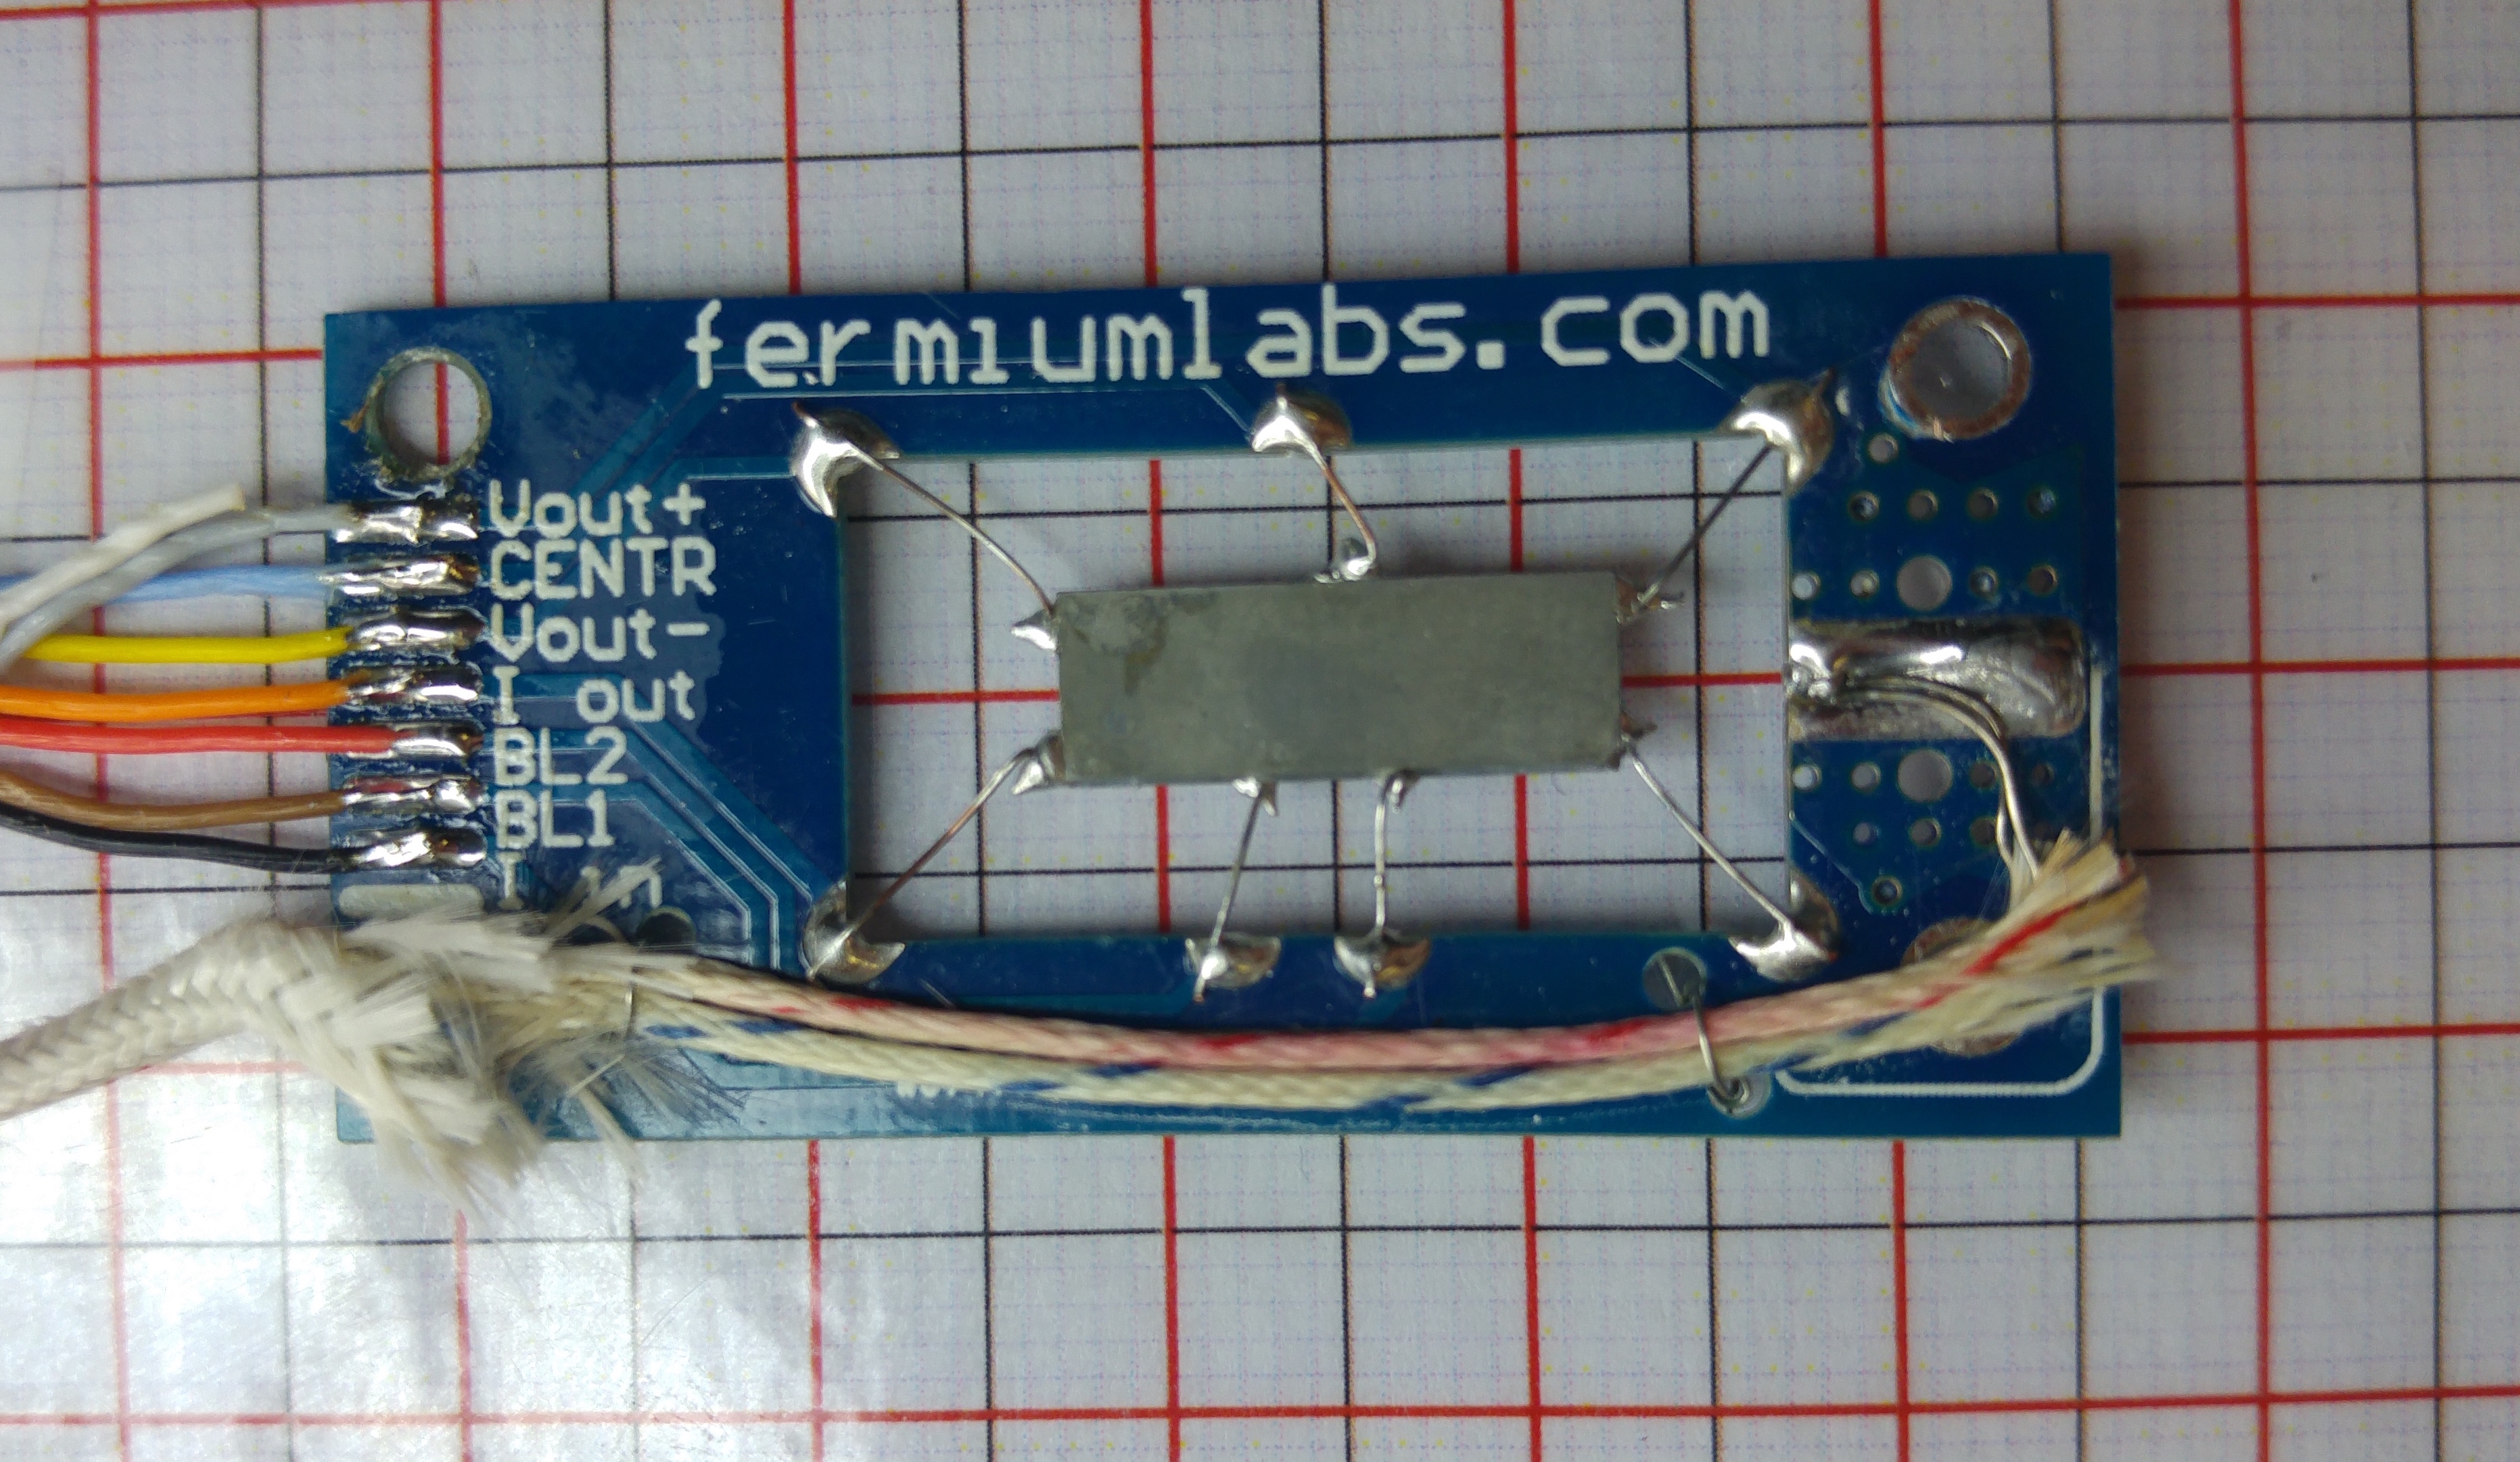
\includegraphics[width=0.65\linewidth]{Assets/Figures/sample_pcb} 

}

\caption{Printed circuit board with germanium sample and thermocuple}\label{fig:sample-pcb}
\end{figure}

The DA outputs are amplified by Programmable Gain Amplifiers (PGA for
short) whose outputs are referred to ground voltage in order to feed the
signals to a data-logger.

The numbering of the contact on the sample corresponds to the number of
the pins in the rj45 connector of the sample assembly.

The two DAs have fixed gains \(G\), set to \(0.5\) for \(V_{out \, R}\)
and to \(10\) for \(V_{out \, H}\) \footnote{The gain can change due to
  specifications and calibration. Please refer to the values displayed
  on the front panel.}, and they're powered from a \(\pm 15V\) power
supply.

\begin{figure}

{\centering 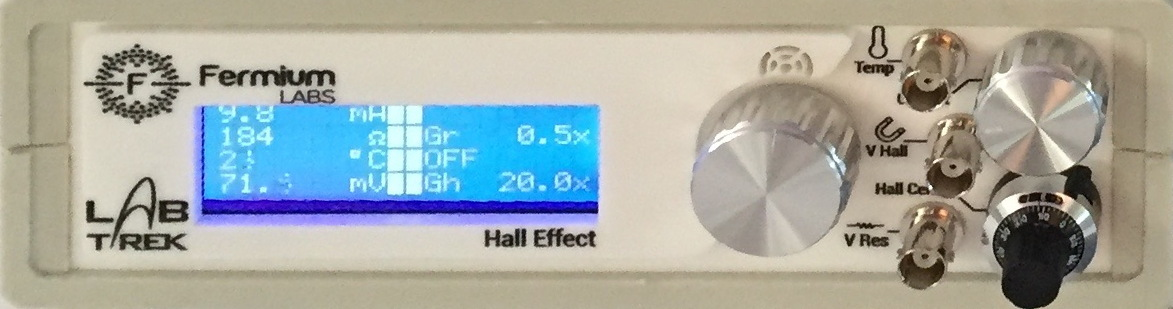
\includegraphics[width=0.65\linewidth]{Assets/Figures/imageFrontPanel0} 

}

\caption{Device front panel}\label{fig:frontPanel}
\end{figure}

The PGA gains are selectable among the following values
\(G_{ PGA}= \{ 1,2,5,10,20,50,100,200\}\) through the front panel as
shown in Fig. \ref{fig:frontPanel}. The gain values shown on the front
panel are the product of DA and PGA gains for both channels.

The output voltages on the front panel are restrained in a number of
cases:

\begin{itemize}
\tightlist
\item
  If the input voltage is \(V_{out} > \frac{30}{G}\) the DA saturates.
\item
  If the output of the DA is not \(0 < V_{out} < 5.1\) it is clamped
  down by a Schottky diode to prevent damage to the circuitry.
\item
  If the output voltage of a PGA is not \(0 < V_{out} < 5\) the PGA
  saturates
\item
  If the \(I_b\) current is set to values smaller than 7 mA or greater
  than 25 mA a warning message appears (``TOO LOW !'' or ``TOO HIGH !''
  respectively), because the constant current generator does not work
  properly outside of this range.
\end{itemize}

Saturation in any channel gives a warning message (``OVERLOAD'') on the
front panel.

The bias current \(I_b\) is is set by rotating the knob on the front
panel, and its value is measured from the voltage drop across a
\(100 \Omega\) resistor, and displayed on the front panel.

The best value for the bias current is a compromise between the need to
obtain a large \(V_H\) to make measurements precise reducing the SNR
(Signal to Noise Ratio) and a low self-heating of the element due to the
Joule effect: \(V_R\) and \(V_H\) signal are proportional to \(I\) while
the Joule self-heating is \(P=RI^2\)

\section{Hall voltage and resistance measurements at room
temperature}\label{hall-voltage-and-resistance-measurements-at-room-temperature}

With a finite value of magnetic field B orthogonal to the large face of
the sample, we should measure identical values for \(V_H\) (but with
opposite sign) when rotating of \(180\,^{\circ}\) the sample. This
behavior must be tested before proceeding to further measurements: if
reversing the \(B\) direction (i.e.~rotating the sample of
\(180\,^{\circ}\) degrees) different values are measured, the offsets
should be better adjusted using potentiometer P in Fig.
\ref{fig:sample-circuitry}.

The absolute value of \(B\) may be varied by changing the width of the
gap between the magnetic poles (see Fig. \ref{fig:ScrewDevice}). One of
the two permanent-magnets mounted on the soft-steel structure may be
moved horizontally by turning the brass-screw: increasing the gap, the
value of \(B\) decreases.

\begin{figure}

{\centering 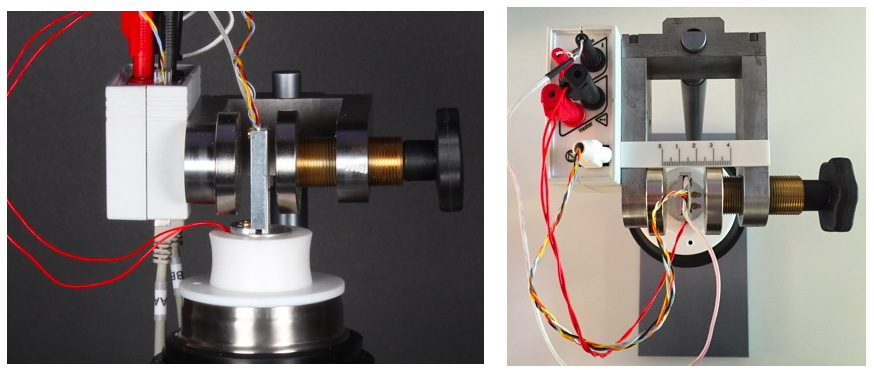
\includegraphics[width=0.65\linewidth]{Assets/Figures/screw_device} 

}

\caption{The screw device for changing the effective magnetic field}\label{fig:ScrewDevice}
\end{figure}

A calibration of the magnetic field \(B\) as a function of the gap \(d\)
may be made using a gauss-meter probe placed between the poles (see Fig.
\ref{fig:BvsGapD})

\section{The set-up for changing and measuring the sample
temperature}\label{the-set-up-for-changing-and-measuring-the-sample-temperature}

The stainless-steel dewar can be filled of liquid nitrogen or a mixture
of acetone and dry-ice (solid carbon dioxyde). The cold finger (the
aluminum bar screwed into the base of the sample) is surrounded by the
liquid nitrogen, allowing the sample to be cooled .

\begin{figure}

{\centering 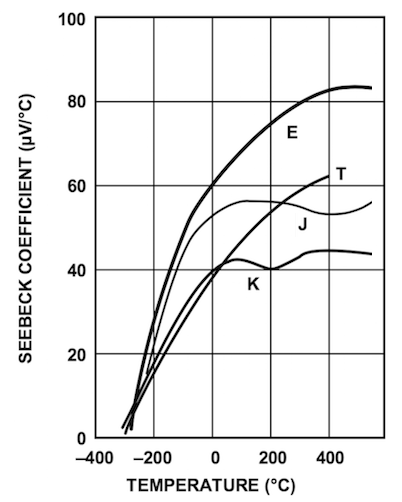
\includegraphics[width=0.3\linewidth]{Assets/Figures/seebeck_coefficient_vs_temperature} 

}

\caption{The thermocouple sensitivity (the Seebeck coefficient) does strongly depend on temperature.}\label{fig:seebeckNonlinearity}
\end{figure}

The temperature is measured by a type K (Chromel-Alumel) thermocouple
thermally coupled to the sample. The small voltage generated by the
thermocouple is amplified by an AD8495\footnote{\href{http://www.analog.com/en/products/amplifiers/specialty-amplifiers/thermocouple-interface-amplifiers/AD8495.html}{AD8495
  datasheet, Analog Semiconductors}} integrated circuit. The output
(roughly proportional to the temperature with a sensitivity of
\(\approx 5\frac { mV }{ \,^{\circ}\mathrm{K} }\) is amplified by a
non-inverting amplifier (not shown in picture) to get
\(\approx 10\frac { mV }{ \,^{\circ}\mathrm{K} }\) and shifted to obtain
\(V_{out \, T}=2.5V\) at
\(273.15\,^{\circ}\mathrm{K}=0\,^{\circ}\mathrm{C}\). While the K type
thermocouple is fairly linear in a small range near room temperature, it
is not linear in the whole temperature range covered by the apparatus,
as can be seen in Fig. \ref{fig:seebeckNonlinearity}.

In order to get a correct measurement it is necessary to compensate for
the non-linearity (see Fig. \ref{fig:seebeckNonlinearity}) of the
thermocouple using the following polynomial:

\begin{equation}
t_{calc}=d_{ 0 }+d_{ 1 }E+d_{ 2 }E^{ 2 }+...+d_{ n }E^{ n }
\label{eq:compensatingPolynomial}
\end{equation}

where \(E\) is the output voltage of the thermocouple in \(mV\).

A fitting polynomial \eqref{eq:compensatingPolynomial} of the fifth order
is sufficient, given the precision of our equipment.

The table \ref{tab:kcoefftable} shows the polynomial coefficients
obtained from a best fit of the NIST\footnote{NIST t-90 tables for K
  type thermocouples,
  \url{http://srdata.nist.gov/its90/download/type_k.tab}} data tables.

\begin{table}

\caption{\label{tab:kcoefftable}Polynomial coefficients obtained from NIST K thermocouple tables ($-200< t \, [^{\circ}\mathrm{C}] <200$).}
\centering
\begin{tabular}[t]{lr}
\toprule
Coefficient & Value\\
\midrule
\$d\_0\$ & 0.383700\\
\$d\_1\$ & 25.220000\\
\$d\_2\$ & 0.279500\\
\$d\_3\$ & 0.072050\\
\$d\_4\$ & 0.014090\\
\$d\_5\$ & 0.001056\\
\bottomrule
\end{tabular}
\end{table}

Fig. \ref{fig:NISTfit} shows the NIST \(t(E)\) data for K thermocouple
compared with the results obtained using eq. 24 and the coefficient of
table 1, and the residual errors in the range
(\(-200< t \, [^{\circ}\mathrm{C}] <200\))

\begin{figure}

{\centering 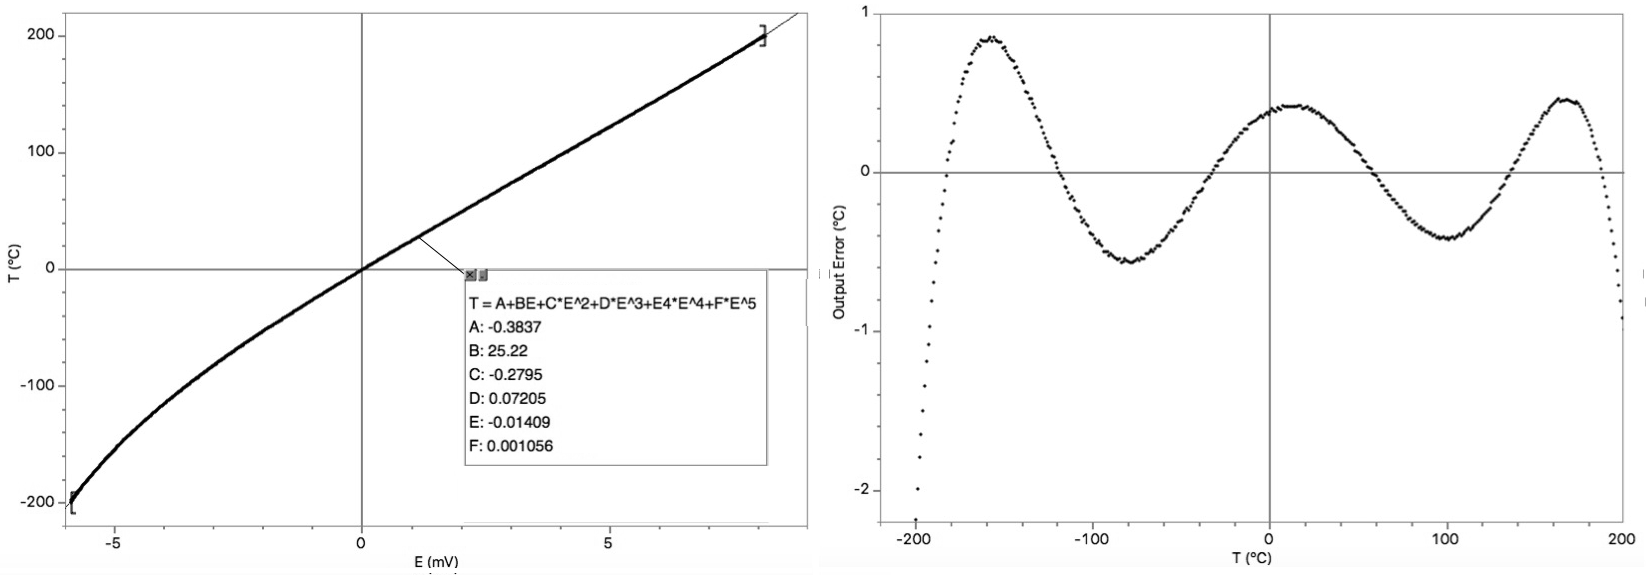
\includegraphics[width=0.65\linewidth]{Assets/Figures/NISTfit} 

}

\caption{Best fit curve for NIST data and residual errors}\label{fig:NISTfit}
\end{figure}

The voltage \(E\) at the thermocouple junction can be obtained\footnote{\href{http://www.analog.com/Assets/Figures/en/technical-documentation/application-notes/AN-1087.PDF}{AN-1087,
  Analog Semiconductors}} from the following equation:

\begin{equation}
E=\frac { 1 }{ 2 } \frac {  V_{ outT }-{ V }_{ Ref }-{ V }_{ Offset } }{ Gain } 
\label{eq:voltageAtThermocoupleJunction}
\end{equation}

where \(V_{outT}\) is the output of the instrument (on the front panel),
\(V_{Ref}=2.5V\) the voltage that indicates a temperature
\(T=0\,^{\circ}\mathrm{C}\), \(V_{offset}\) is the error voltage at
\(0\,^{\circ}\mathrm{C}\) to achieve 125 mV at
\(25\,^{\circ}\mathrm{C}\) and \(Gain\) is the internal gain of the
AD8495 amplifier.

Using the fitting polynomial \eqref{eq:compensatingPolynomial} allows us
to finally obtain the temperature in Celsius:

\begin{equation}
t={ f }_{ comp }\left( E \right)
\label{eq:FcompE}
\end{equation}

\begin{equation}
t={ f }_{ comp } \left( \frac { 1 }{ 2 } \frac { V_{ out }-2.5-1.25\cdot 10^{ -3 } }{ 122.4 } \right)
\label{eq:ad8494Compensated}
\end{equation}

A digitally controlled resistive element (heater) is wound around the
base of the sample, allowing to heath it up after reaching room
temperature. The instruments automatically shuts down the heater if
\(t \ge 170\, \,^{\circ}\mathrm{C}\).

\clearpage 

\section{Suggested procedure}\label{suggested-procedure}

The display on the controller box shows the sample temperature in
Celsius (calculated from the measured thermocouple signal), the measured
bias current \(I_b\) (mA), the sample resistance (calculated from the
measured voltage drop across the sample) and the selected values of the
\(V_H\) and \(V_R\) channels.

To obtain accurate measurements the best procedure is the following:

\begin{enumerate}
\def\labelenumi{\arabic{enumi}.}
\item
  Connect the sample cables to the HUB and the HUB to the controller
  with the two ethernet cables (note: connect the controller port A with
  HUB port A ,and B with B).

  Connect all the controller outputs (BNC ports) to your data-logger
  sensor inputs and choose an acquisition run with approximately
  \(0.1Hz\) rate (i.e.~1 sample every 10 seconds) and duration at least
  6000 seconds.
\item
  Choose a width for gap between the permanent magnets and measure the
  magnetic field B in the middle, using a gauss-meter. Place the sample
  far from the magnetic field and trim the balance-potentiometer to
  minimize the \(V_H\) signal. Lock the potentiometer knob.
\item
  Place the sample in the middle of the gap. Choose a proper value for
  the current \(I_b\) within the 7-25 mA allowed range, and select the
  proper gains for \(V_H\) and \(V_R\) channels. Note : the resistance
  at higher temperature may exceed the value at room temperature by a
  factor 2, and also the VH signal increase with temperature. Therefore
  at room temperature your data-logger should read typically
  \(V_{out \, H} <0.4V\) and \(V_{out \, R}<2.5V\).
\item
  Check that the \(V_H\) value changes sign when rotating the sample of
  180° around vertical axis. Choose the orientation that gives positive
  \(V_H\).
\item
  Prepare all the data conversion you think useful. For example : from
  \(V_{out \, R}\) and the known \(I_b\) and \(G_R\) gain values obtain
  R(ohm), from \(V_{out \, H}\) and \(G_H\) gain values obtain \(V_H\)
  (in \(mV\)), from \(V_{out \, T}\) obtain the K-thermocouple e.m.f.
  E(mV)
  \([E=0.5 \cdot 1000 \cdot \frac{ (V_{out \, T}-2.5-0.00125)}{122.4}]\),
  from the calculated \(E(mV)\) obtain the Celsius temperature \(t\)
  using the fitting polynomial,\ldots{}
\item
  Fill about half of the dewar with liquid nitrogen and wait until the
  liquid surface is quiet.
\item
  Prepare at least one graph with temperature vs time, and one with
  output signals vs time in your data-logger. Insert the cold finger
  into the dewar (the PTFE dewar-cover should seat stable onto the dewar
  mouth, and the PTFE heater cover should be set with the hole hosting
  the pin protruding from the dewar-cover) as shown in Fig.
  \ref{fig:ScrewDevice}. Adjust the sample in the mid of the magnet-gap
  and start the data acquisition.
\item
  When the plot temperature vs time shows a slope close to zero, stop
  the data acquisition and save your data.
\item
  Empty the dewar (e.g.~transferring the residual liquid nitrogen into
  another dewar), reposition the sample in the middle of the magnets-gap
  and start a new data acquisition for increasing temperature.
\item
  When the temperature vs.~time slope start approaching zero, switch-ON
  the heater (Press the control knob 3 times, until the arrow reaches
  the OFF and turn the knob).
\end{enumerate}

To obtain precise measurements, at least one hour is required for the
whole temperature sweep.

Note: it is not suggested to keep liquid nitrogen inside the dewar while
heating-up the sample: the temperature would rise more slowly and more
humidity would condense onto the outer surface of the aluminum probe
envelope.

It is also useful to blow-off the frost in order to prevent water
entering the probe envelope (this might affect the thermocouple signal).

\section{Typical results}\label{typical-results}

The sample shown in figure 3 (and used to obtain the data in the
following examples) has thickness \(t=0.5mm\), width \(w=10mm\) and
lenght \(l=15mm\).

A calibration of the magnetic field intensity \(B\) vs.~gap \(d\)
between magnets is shown in Fig. \ref{fig:BvsGapD}.

\begin{figure}

{\centering 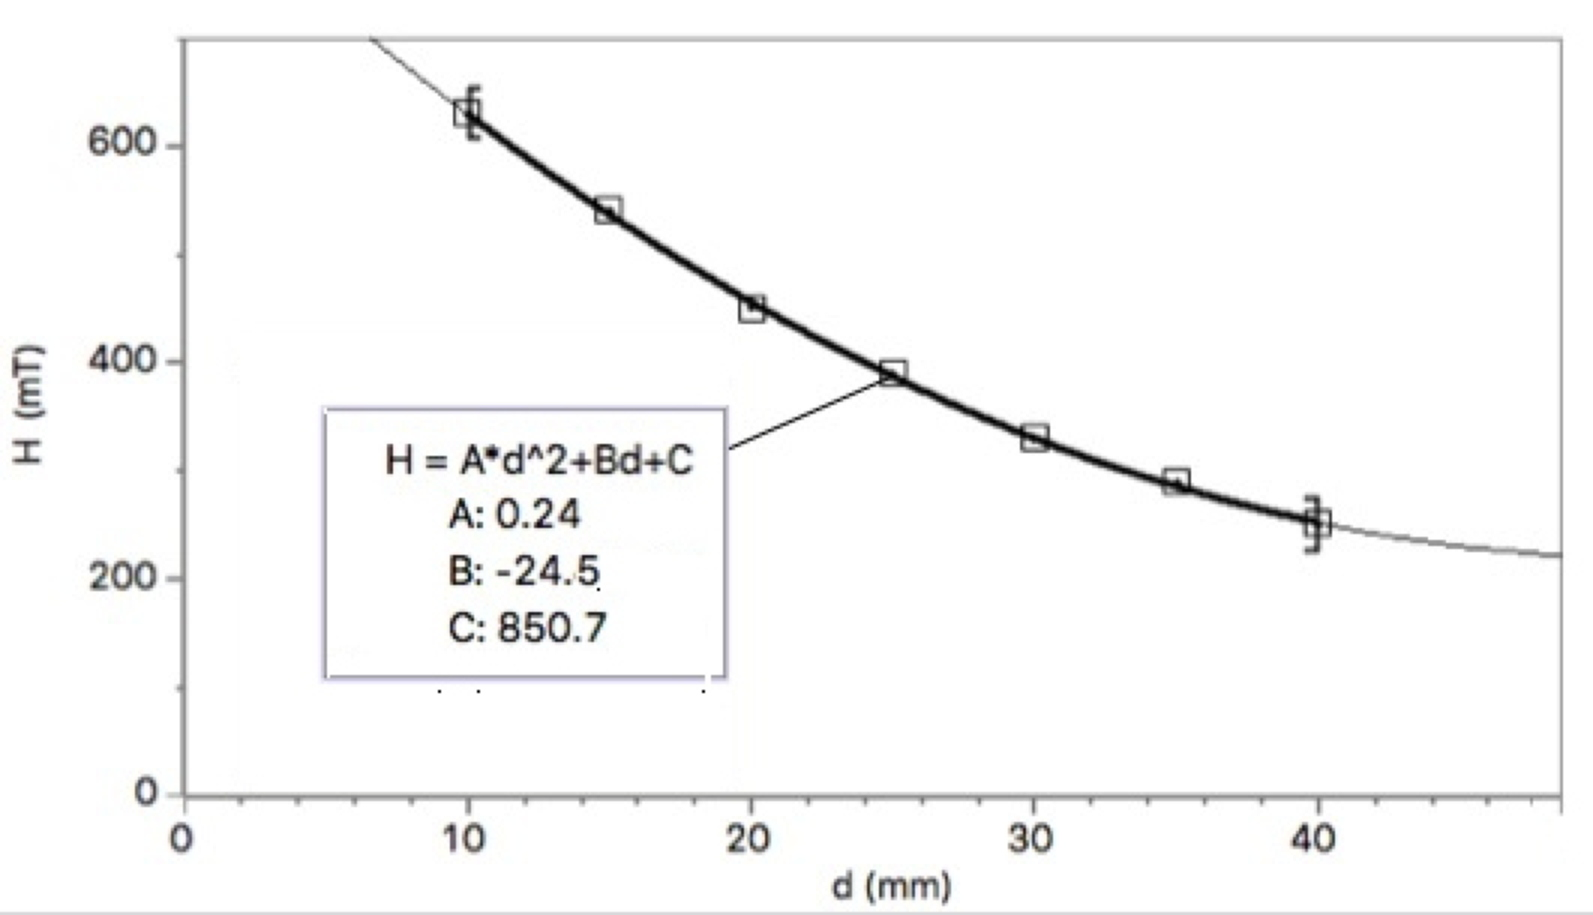
\includegraphics[width=0.65\linewidth]{Assets/Figures/H_vs_d} 

}

\caption{Measured $B$ values vs gap width $d$}\label{fig:BvsGapD}
\end{figure}

An example of the measured \(V_H\) vs.~magnetic field \(B\) at room
temperature is shown in Fig. \ref{fig:HallvsIb}.

\begin{figure}

{\centering 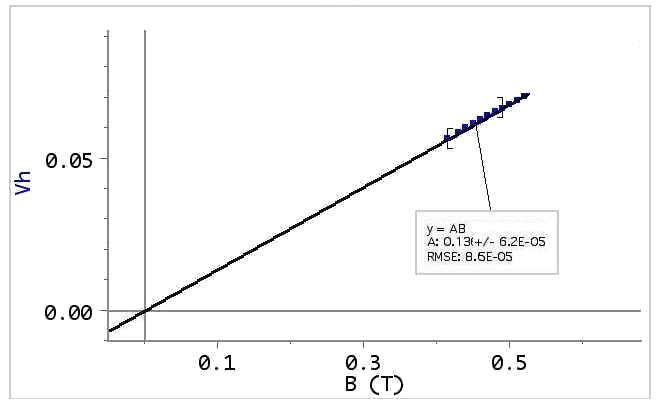
\includegraphics[width=0.65\linewidth]{Assets/Figures/Vh_vs_B} 

}

\caption{Hall voltage versus magnetic field intensity $B$}\label{fig:HallvsIb}
\end{figure}

Fig. \ref{fig:Output-voltages-versus-time} shows an example of the
measured values of the 3 output signals vs temperature obtained with a
constant bias current \(I_B=10mA\) and in a 0.4 \(T\) magnetic field,
using Vernier-LabPro interface. The graph shows \emph{Potential 1}
\(= V_{out \, T}\), \emph{Potential 2} \(= V_{out \,H}\),
\emph{Potential 3} \(= V_{out \, R}\).

\begin{figure}

{\centering 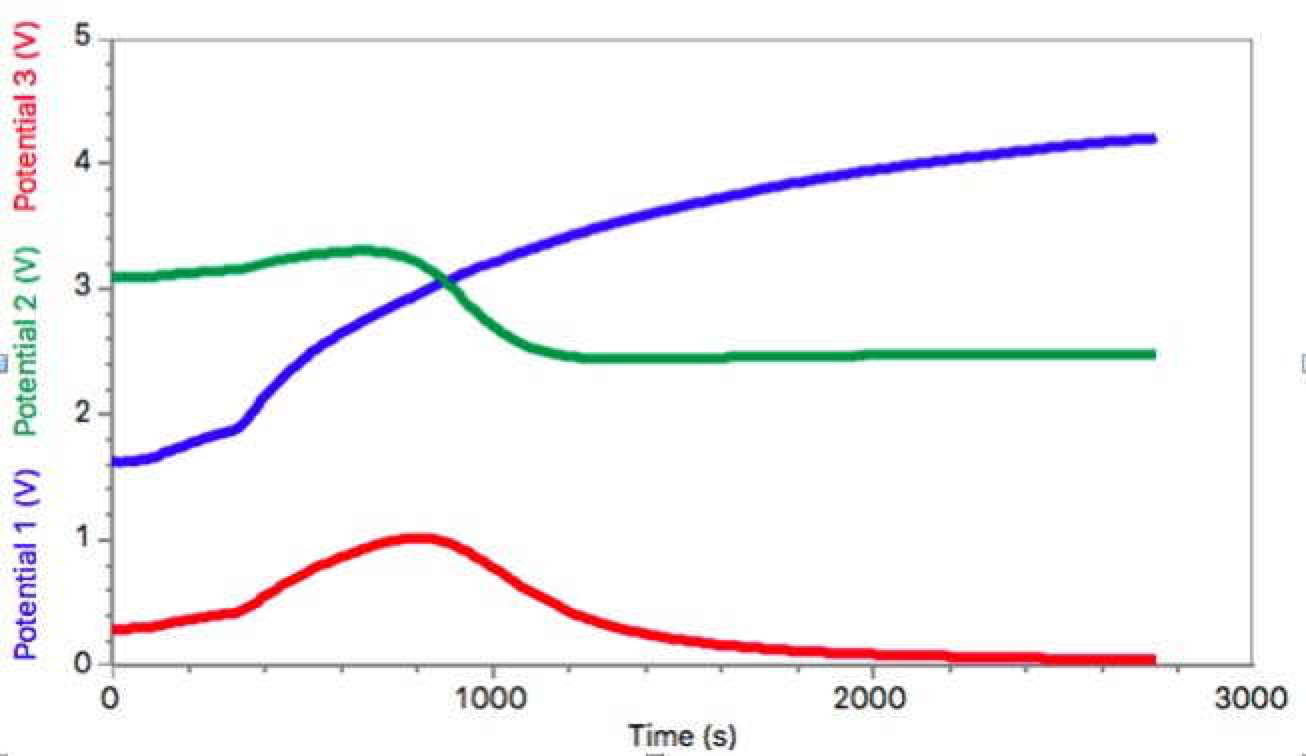
\includegraphics[width=0.65\linewidth]{Assets/Figures/Out_vs_time} 

}

\caption{Output voltages versus time}\label{fig:Output-voltages-versus-time}
\end{figure}

Fig. \ref{fig:Example} shows an example of calculated data obtained
using LoggerPro software. The Hall voltage \(V_{H}\) (in mV) is is
obtained from \(V_{outH}\) by subtracting the offset 2.5 V and by
accounting for the used value of the channel-H gain (here GainH=10). The
resistance \(R\) is calculated from \(V_{outR}\) by accounting for the
used value of the channel-R gain (here GainR=0.5)and the measured value
of the bias current \(Ib\) .

\begin{figure}

{\centering 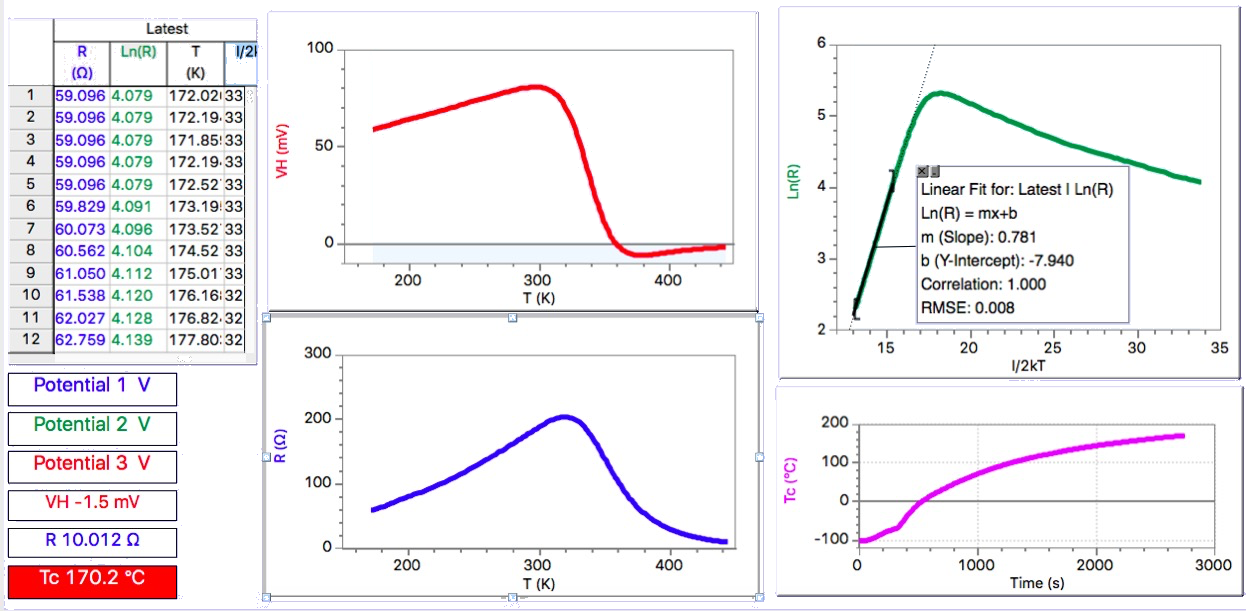
\includegraphics[width=0.65\linewidth]{Assets/Figures/example} 

}

\caption{Example of calculated data}\label{fig:Example}
\end{figure}

In order to evaluate the Ge energy gap \(E_g\), a plot of \(ln(R)\) vs.
\(1/2kT\) was built, after calculating from the Celsius temperature
\(Tc\) the absolute temperature \(T\) (\(k\) is the Boltzmann constant
\(k = 8.617 \cdot 10^{-5}\).

From the slope in the intrinsic region (high temperature region, see
Fig. \ref{fig:EgFit} ) we get the value of the energy gap \(E_g\),
extrapolated linearly to \(T=0^{\circ}\mathrm{K}\), that can be compared
to the known value for germanium (\(E_g^o=0.78\), see Appendix 3)

\begin{figure}

{\centering 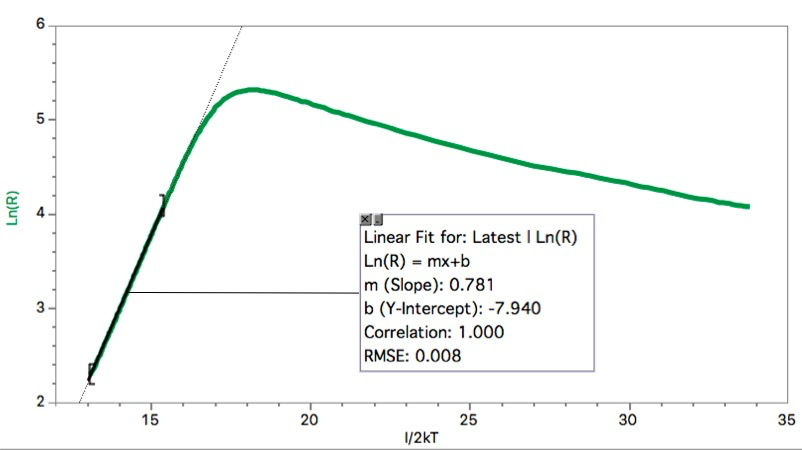
\includegraphics[width=0.65\linewidth]{Assets/Figures/ImageEgFit} 

}

\caption{Example of linear best fit in the intrinsic region (high temperature)}\label{fig:EgFit}
\end{figure}

\chapter{Appendix 1: Use of the optional Extension
HUB}\label{appendix-1-use-of-the-optional-extension-hub}

An optional Extension HUB (ExtHUB)is provided with the device. This
allows the user to measure the voltages (with respect to the ground or
as differential voltages) at the 7 contacts on the Ge sample, by using
an high impedance multimeter.

The ExtHUB must be connected between the sample and the fixed HUB
(FixHUB) placed on the magnet holder using the black cable with rj45
plugs. Note: do not unplug the cable from the ExtHUB; the cable should
be connected to the FixHUB and the sample cable should be connected to
the ExtHUB (see Fig. \ref{fig:ExtensionHUB}).

\begin{figure}

{\centering 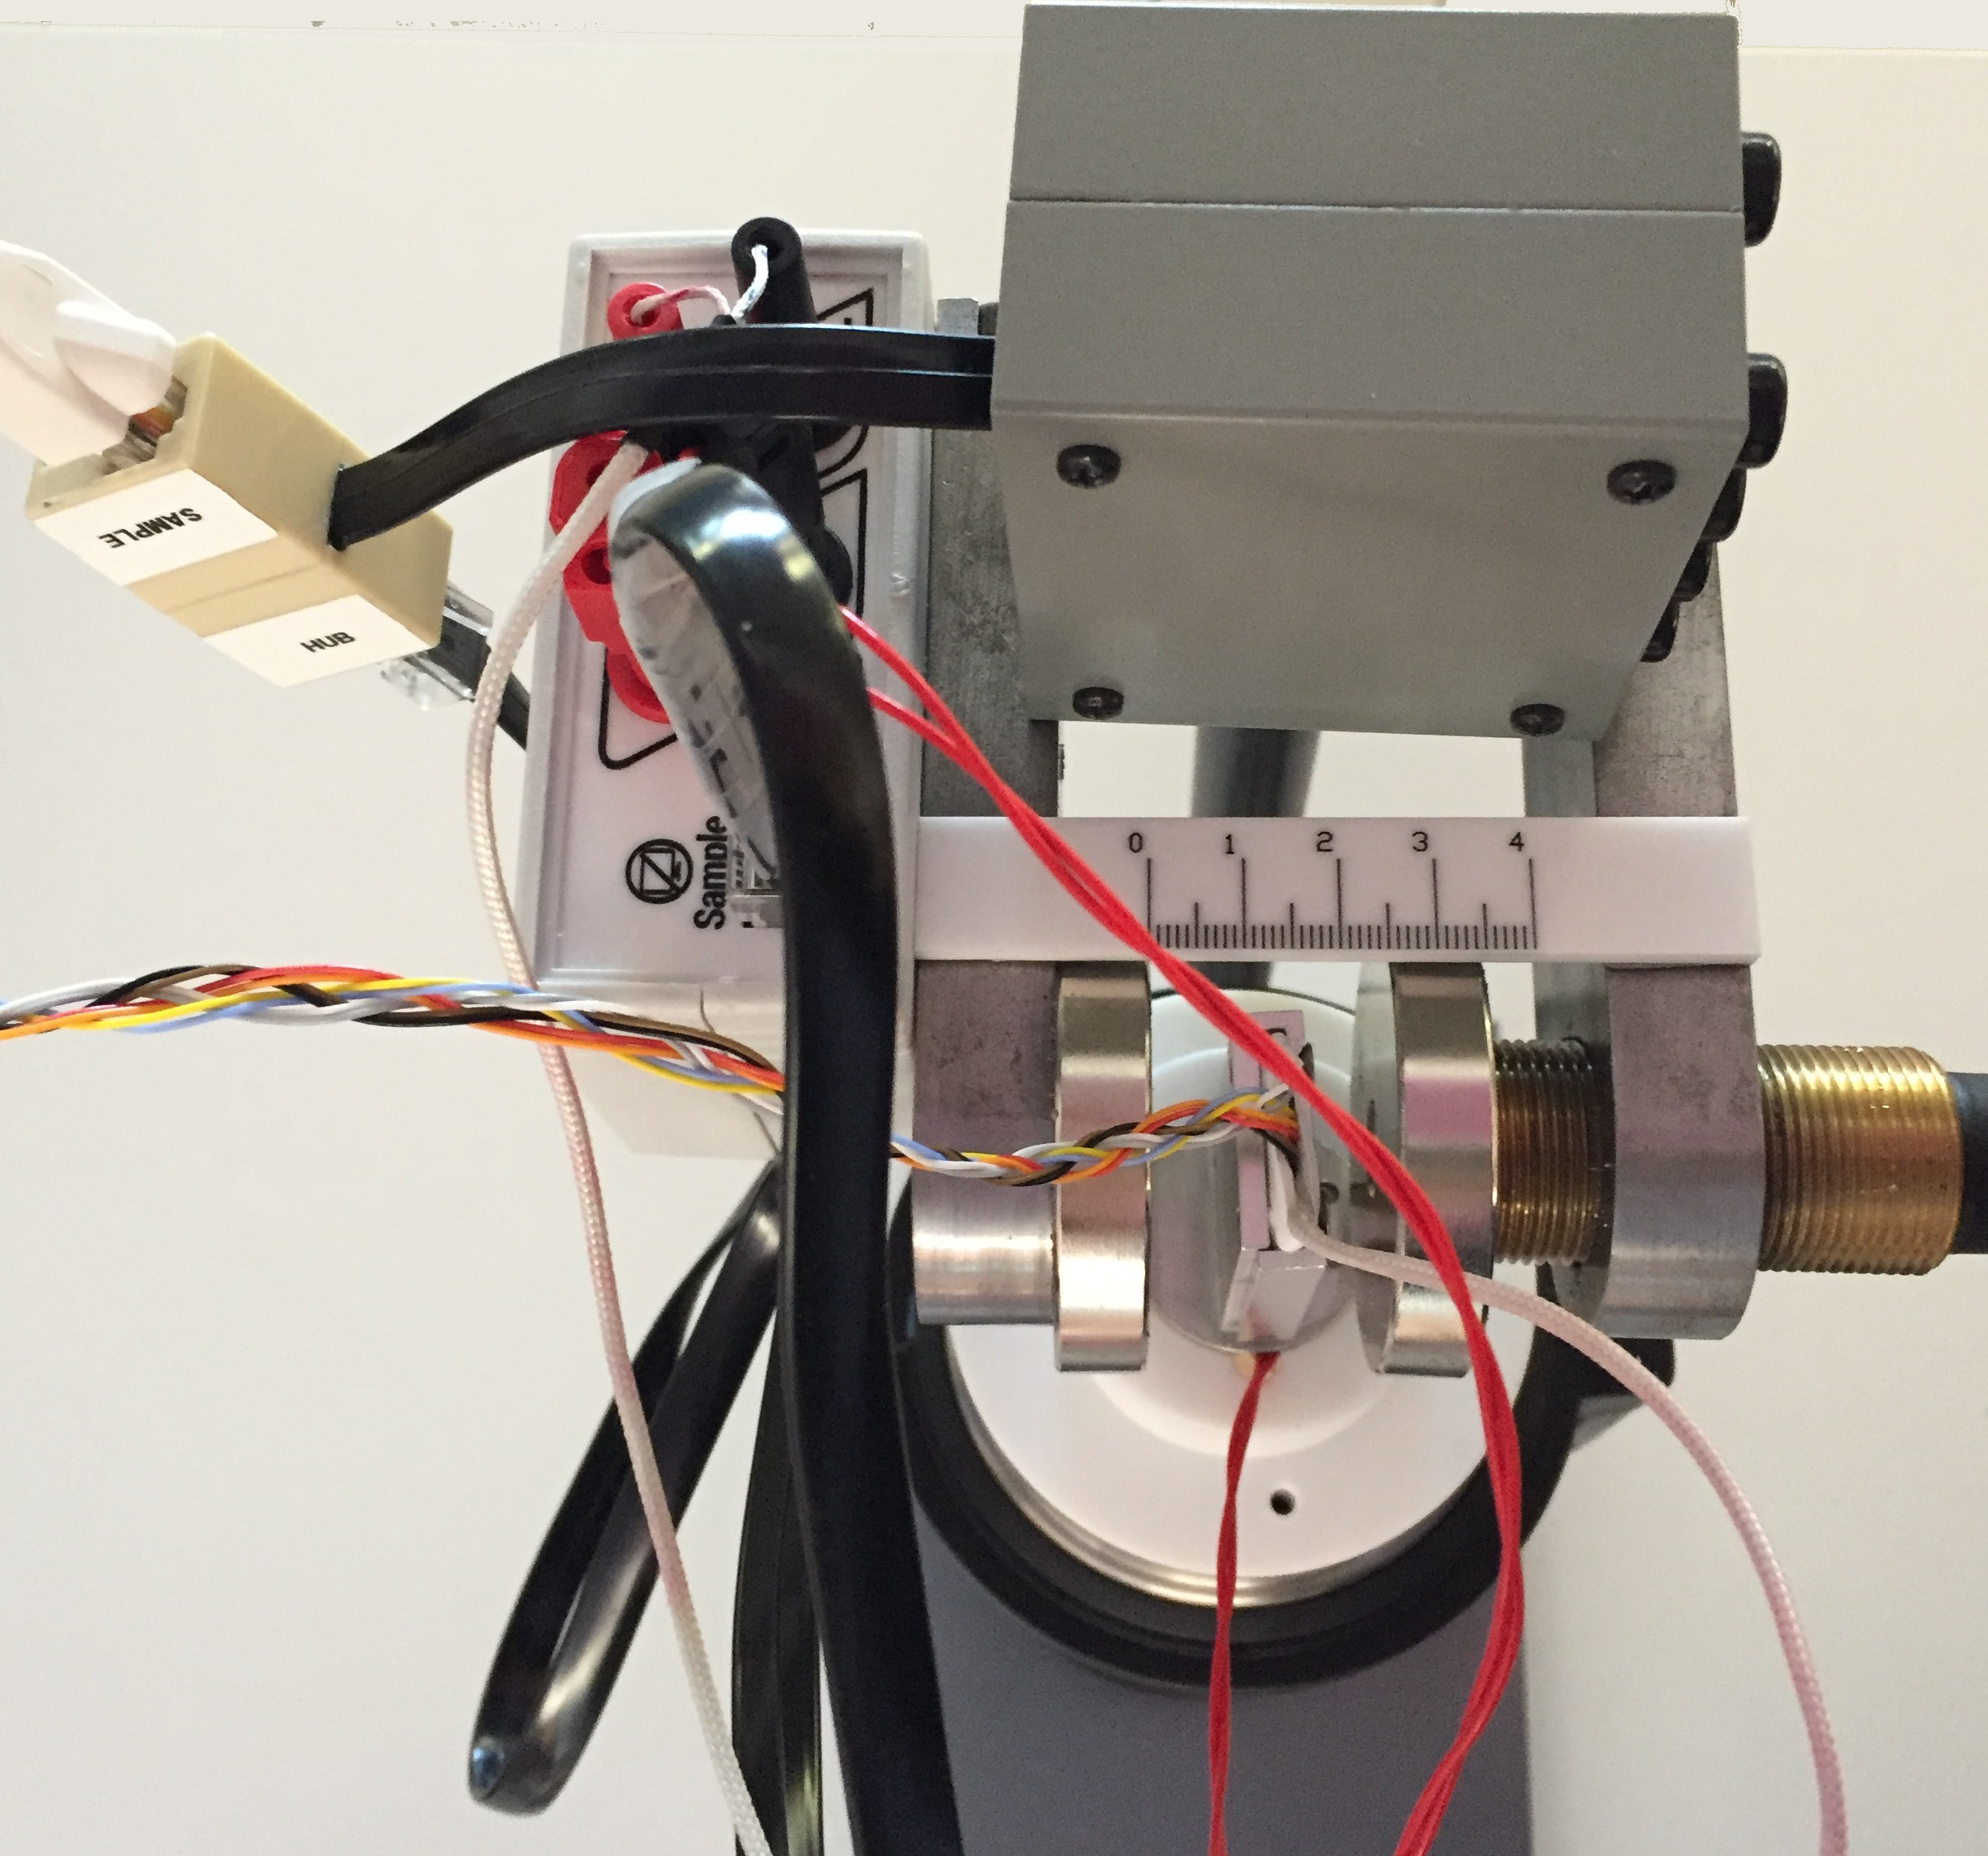
\includegraphics[width=0.4\linewidth]{Assets/Figures/imageExtensionHub} 

}

\caption{The Extension HUB connections}\label{fig:ExtensionHUB}
\end{figure}

For example a two-wire resistance measurement between the Test Points
(TP) 1-4, 1-5, 7-4 or 7-5 will give a value larger than the real
resistance measured by the 4-contacts method, and displayed on the front
panel.

Note: be sure to switch-off the controller while taking measurements
with the ExtHUB !

\chapter{\texorpdfstring{Appendix 2: calculation of \(R_H\) for small
and high magnetic
field}{Appendix 2: calculation of R\_H for small and high magnetic field}}\label{appendix-2-calculation-of-r_h-for-small-and-high-magnetic-field}

The motion equation \((F=ma)\) for charge carriers can as well be
written as:

\begin{equation}
m(\frac{dv}{dt}+\frac{v}{\tau}) = qE+ q\vec{v} \wedge \vec{B} 
\label{eq:MotionEquationForChargeCarriers}
\end{equation}

where the charge \(q\) is the \(\pm e\) for holes and electrons and we
account for the mean time \(\tau\) between collisions and for the
Lorentz force. In stationary conditions the acceleration is zero.
Therefore the velocities along \(x\) (\(B\) is directed along \(z\)) for
electrons and holes are respectively:

\begin{equation}
V_{ex}=-\frac{e\tau}{m}E_x+\frac{e\tau}{m}\vec{v}\wedge\vec{B}=-\mu_e v_{e\, y}B
\label{eq:XvelocitiesForElectrons}
\end{equation}

\begin{equation}
V_{hx}=\mu_h E_x+\mu_h v_{e\, x}B
\label{eq:XvelocitiesForHoles}
\end{equation}

And, for velocities along y:

\begin{equation}
V_{ e \, y} = -\mu_e E_y- \mu_e V_{e \, x} B
\label{eq:YvelocitiesForElectrons}
\end{equation}

\begin{equation}
V_{h \, y} = \mu_h E_y + \mu_h v_{h \, x}B
\label{eq:YvelocitiesForHoles}
\end{equation}

The current density along the \(x\) axis
\((J = e V_{h \, x} P - eV_{e \quad x} n)\) can as well be written as:

\begin{equation}
J_x \approx e(p \mu_h + n \mu_e)E_x + e(p \mu_h v \mu_{h \, y} - n \mu_e v_{e \, y})B \approx \\
\approx e ( p \mu_h + n \mu_e) E_x + e (p \mu_h^2 -n \mu_e^2 )BE_y
\label{eq:currentDensityAlongX}
\end{equation}

where we made the approximation \(v_y \approx \mu_y E_y\), neglecting
here the Lorentz force. Recalling that \(E_y \ll E_x\), for small
magnetic fields \(B\) \eqref{eq:currentDensityAlongX} may be approximated
by:

\begin{equation}
J_x \approx e(p \mu_h + n \mu_e) E_x
\label{eq:currentDensityAlongXaproxymated}
\end{equation}

For negligible current density along y we have:

\begin{equation}
J_y = e p v_{h \, y} - env_{e \, y} = 0
\label{eq:currentDensityAlongYNegligible}
\end{equation}

or using \(v_{h \, x}\) and \(V_{e \, x}\) definitions:

\[J_y = ep ( \mu_h E_y + \mu_h v_{h \, x} B) - en( -\mu_e E_y - \mu_e v_{e \, x}B) = 0\]

\[e(p \mu_h + n \mu_e) E_y + e(p \mu_h v_{h \, x} + n \mu_e v_{e \, x}) B = 0\]

\[E_y = B \frac {p \mu_h v_{h \, x} + n \mu_e v_{e \, x}}{p \mu_h + n \mu_e}\]

If again we assume \(v_x \approx \mu_xE_x\) (neglecting, for small B,
the correction for the Lorentz force we can write:

\[E_y \approx B \frac{p \mu^2_h - n \mu^2_e}{p \mu_h + n \mu_e} E_x\]

In this way the Hall coefficient becomes:

\begin{equation}
R_H = - \frac{E_y}{J_x B_z} \approx \frac {p \mu^2_h - n \mu_e^2}{e (p \mu_h + n \mu_e )^2}
\label{eq:hallCoefficientBecomes}
\end{equation}

The formula \eqref{eq:hallCoefficientBecomes} holds true only for
\emph{small values} of \(B\). For large \(B\) values we must use
\eqref{eq:hallCoefficientBecomes} for \(J_x\) the definition
\eqref{eq:currentDensityAlongX} instead of
\eqref{eq:currentDensityAlongXaproxymated}, obtaining for the Hall
coefficient \(R_H\):

\begin{equation}
R_{ H }(B)=\frac { E_{ y } }{ BJ_{ x } } \approx \frac { \left[ B\frac { (p\mu ^{ 2 }_{ h }-n\mu ^{ 2 }_{ e }) }{ (p\mu _{ h }+n\mu _{ e }) } E_{ x } \right] }{ Be\left[ (p\mu _{ h }+n\mu _{ e })+B^{ 2 }\frac { (p\mu ^{ 2 }_{ h }-n\mu ^{ 2 }_{ e })^{ 2 } }{ (p\mu _{ h }+n\mu _{ e }) } \right] { E }_{ x } } = \\
=\frac { (p\mu ^{ 2 }_{ h }-n\mu ^{ 2 }_{ e }) }{ e(p\mu _{ h }+n\mu _{ e })^{ 2 }\left[ 1+B^{ 2 }\frac { (p{ \mu }_{ h }^{ 2 }-n\mu ^{ 2 }_{ e })^{ 2 } }{ (p\mu _{ h }+n\mu _{ e })^{ 2 } } \right] } =\frac { R_{ H(B=0) } }{ 1+KB^{ 2 } }
\label{eq:HallCoefficientBigEquation}
\end{equation}

which tends to saturate at high B values.

\clearpage

\chapter{\texorpdfstring{Appendix 3: Temperature dependence of
\(E_g\)}{Appendix 3: Temperature dependence of E\_g}}\label{appendix-3-temperature-dependence-of-e_g}

Experimental results consistently shows that the energy gap depends on
temperature and for Germanium we can find in the literature the
following empirical law:

\begin{equation}
E_{ g }(T)=0.742-\frac { 4.8\cdot 10^{ -4 }T^{ 2 } }{ T+235 } \quad \quad [eV]
\label{eq:eGempiricalLaw}
\end{equation}

This may be approximated, in the high temperature region, by a linear
law as follows:

\[E_g (T) = A \cdot BT\]

where the constants \(A\) is the value of \(E_g\) \emph{linearly
extrapolated} to \(T=0\): \[E^0_g = A = 0.78eV\]

Since in the intrinsic region (high temperature) the resistance depends
on the absolute temperature \(T\) as \(exp( \frac{E_G}{2kT})\), a plot
of \(ln( R )\) vs \(\frac{1}{2 K T}\) using a linear approximation for
\(E_g(T)\) results in a straight line with slope \(E^0_g\)

\begin{figure}

{\centering 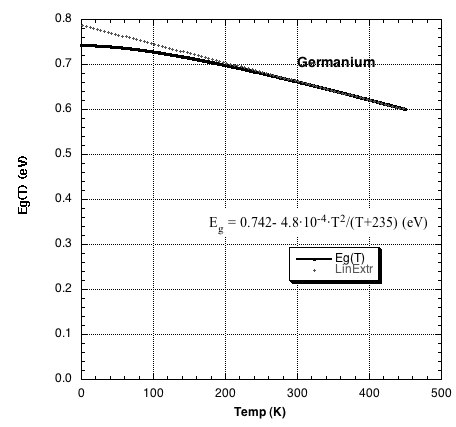
\includegraphics[width=0.65\linewidth]{Assets/Figures/Eg_vs_T} 

}

\caption{Temperature dependance of the energy gap}\label{fig:EgTdependance}
\end{figure}

\clearpage

\chapter{Warnings}\label{warnings}

\textbf{Using high magnetic field require some caution:}

\begin{itemize}
\item
  You must avoid approaching any magnetizable object (clocks, electronic
  devices, screwdrivers\ldots{}), which when brought too close may be
  permanently magnetized.
\item
  A pinch hazard subsists if steel or other ferromagnetic material gets
  close to the magnets.
\item
  Do not attempt to unscrew the magnets.
\item
  The Magnets are brittle. A rapid shock with another magnet or
  ferromagnetic material may release shards dangerous for the eye.
\item
  The apparatus \textbf{MUST NOT} be used by people with pacemakers.
\end{itemize}

\clearpage

\chapter{References}\label{references}

\begin{itemize}
\tightlist
\item
  J.C. Slater \emph{Quantum Theory of matter}, mcGraw-Hill 1951.
\item
  C.L.Chin e C.R.Westgate, \emph{The Hall Effect and Its Applications},
  Plenum Press, NY, 1979
\item
  J.R.Hook, H.E.Hall \emph{Solid State Physics}, John Wiley \&Sons 1991.
\item
  A. C. Melissinos \emph{Experiments in modern Physics}, Academic Press,
  1993.
\item
  \emph{New Semiconductor materials. Characteristics and Properties},
  \newline \url{http://www.ioffe.ru/SVA/NSM/Semicond/Ge/index.html}
  (Electronic archive)
\item
  \emph{The Semiconductor informations WebSite} (properties of
  Germanium),
  \newline \url{http://www.semiconductors.co.uk/propiviv5431.htm}
\end{itemize}

\chapter{Authorship}\label{authorship}

This Handbook was originally written by Giacomo Torzo of
\href{http://labtrek.it}{Labtrek}

Integrations by Davide Bortolami and Statistical analysis by Simone
Tosato of \href{http://fermiumlabs.com}{Fermium LABS}

\section{Revision history}\label{revision-history}

For a complete revision history, check out the
\href{https://github.com/fermiumlabs/Hall-effect-apparatus/commits/master}{Github
repository}.

The last version of this document can be downloaded at
\href{https://frm.li/hallhandbookmaster}{frm.li/hallhandbookmaster} or
with the following QR code:

\begin{figure}
\centering
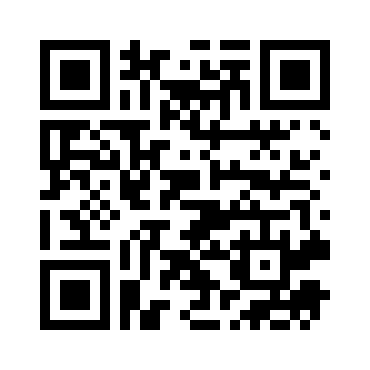
\includegraphics[width=0.40000\textwidth]{Assets/Figures/qr_last.jpg}
\caption{}
\end{figure}


\end{document}
